\documentclass[12pt]{article}
\usepackage{geometry}                % See geometry.pdf to learn the layout options. There are lots.
\geometry{letterpaper}                   % ... or a4paper or a5paper or ... 
%\geometry{landscape}                % Activate for for rotated page geometry
\usepackage[parfill]{parskip}    % Activate to begin paragraphs with an empty line rather than an indent
\usepackage{daves,fancyhdr,natbib,graphicx,dcolumn,amsmath,lastpage,url}
\usepackage{amsmath,amssymb,epstopdf,longtable}
\usepackage{paralist}  % need to properly formulate standard answer blocks
\usepackage[final]{pdfpages}
\DeclareGraphicsRule{.tif}{png}{.png}{`convert #1 `dirname #1`/`basename #1 .tif`.png}
\pagestyle{fancy}
\lhead{CE 3372 Water Systems Design; Exam 2}
\rhead{Name:\_\_\_\_\_\_\_\_\_\_\_\_\_\_\_\_\_\_\_\_\_\_\_\_\_\_\_\_\_\_\_\_\_\_}
\lfoot{REVISION A}
\cfoot{}
\rfoot{Page \thepage\ of \pageref{LastPage}}
\renewcommand\headrulewidth{0pt}
\newcommand\tab[1][1cm]{\hspace*{#1}}



\begin{document}
%%%%%%%%%%%%%%%%%%%%%%%%%%%%%%%%%%%
\begingroup
\begin{center}
{\textbf{{ CE 3372 Water Systems Design}  \\ Fall 2016} \\
Equation List}
\end{center}
\endgroup

Unit conversions\\
\begin{equation}
1\text{~meter} = 3.28\text{~feet}
\end{equation}
\begin{equation}
1\text{~cubic foot} = 7.48\text{~gallons}
\end{equation}
\begin{equation}
1\text{~kilogram} ~\approx 2.2\text{~pounds}
\end{equation}
\begin{equation}
1\text{~acre} = 43,560\text{~square feet}
\end{equation}
\begin{equation}
1~\frac{\text{newton-meter}}{\text{second}} = 1\text{Watt}
\end{equation}

Modified Bernoulli (Energy) equation.
\begin{equation}
\frac{p_1}{\rho g}+\alpha_1 \frac{V_1^2}{2g} + z_1 + h_p =
\frac{p_2}{\rho g}+\alpha_2 \frac{V_2^2}{2g} + z_2 + h_t + h_l
\end{equation}

Darcy-Weisbach head-loss equation
\begin{equation}
h_l=f \frac{L}{D}\frac{V^2}{2g}
\end{equation}

Hazen-Williams head-loss equation (U.S. Customary)
\begin{equation}
h_f = 3.02~ L~D^{-1.167} (\frac{V}{C_h})^{1.85}
\end{equation}

Jain equation for pressurized pipes (U.S. or S.I.)
\begin{equation}
Q=-2.22D^{5/2} \times \sqrt{gh_f/L}\times[log_{10} (\frac{k_s}{3.7D} + \frac{1.78\nu}{D^{3/2}\sqrt{gh_f/L}} )]
\end{equation}
Jain approximation for friction factor  (U.S. or S.I.)
\begin{equation}
f=\frac{0.25}{[log_{10} (\frac{\frac{k_e}{D}} {3.7} + \frac{5.74}{Re_d^{0.9} } )]  ^2}
\label{eqn:friction-factor-jain}
\end{equation}
Jain approximation for diameter  (U.S. or S.I.)
\begin{equation}
D=0.66[\epsilon^{1.25}\times(\frac{LQ^2}{gh_f})^{4.75}+\nu Q^{9.4}\times(\frac{L}{gh_f})^{5.2}]^{0.04}
%\label{eqn:diameter-jain}
\end{equation}

Manning's equation (U.S. Customary and S.I. units)
\begin{equation}
Q=\frac{1.49}{n} A R^{2/3} S^{1/2}~\text{(U.S. Customary)}
\end{equation}
\begin{equation}
Q=\frac{1.0}{n} A R^{2/3} S^{1/2}~\text{(S.I.)}
\end{equation}

Rational runoff equation (U.S. Customary)
\begin{equation}
Q_{peak}=C \times i \times A
\end{equation}
where $i$ is intensity in inches-per-hour, and $A$ is drainage area in acres.

\begin{tabular}{p{6in}}
~\\ \hline
\end{tabular}

Depth-Area, -Topwidth, -Perimeter for Trapezoidal Channel (both side slopes same)
\begin{figure}[h!] %  figure placement: here, top, bottom, or page
   \centering
   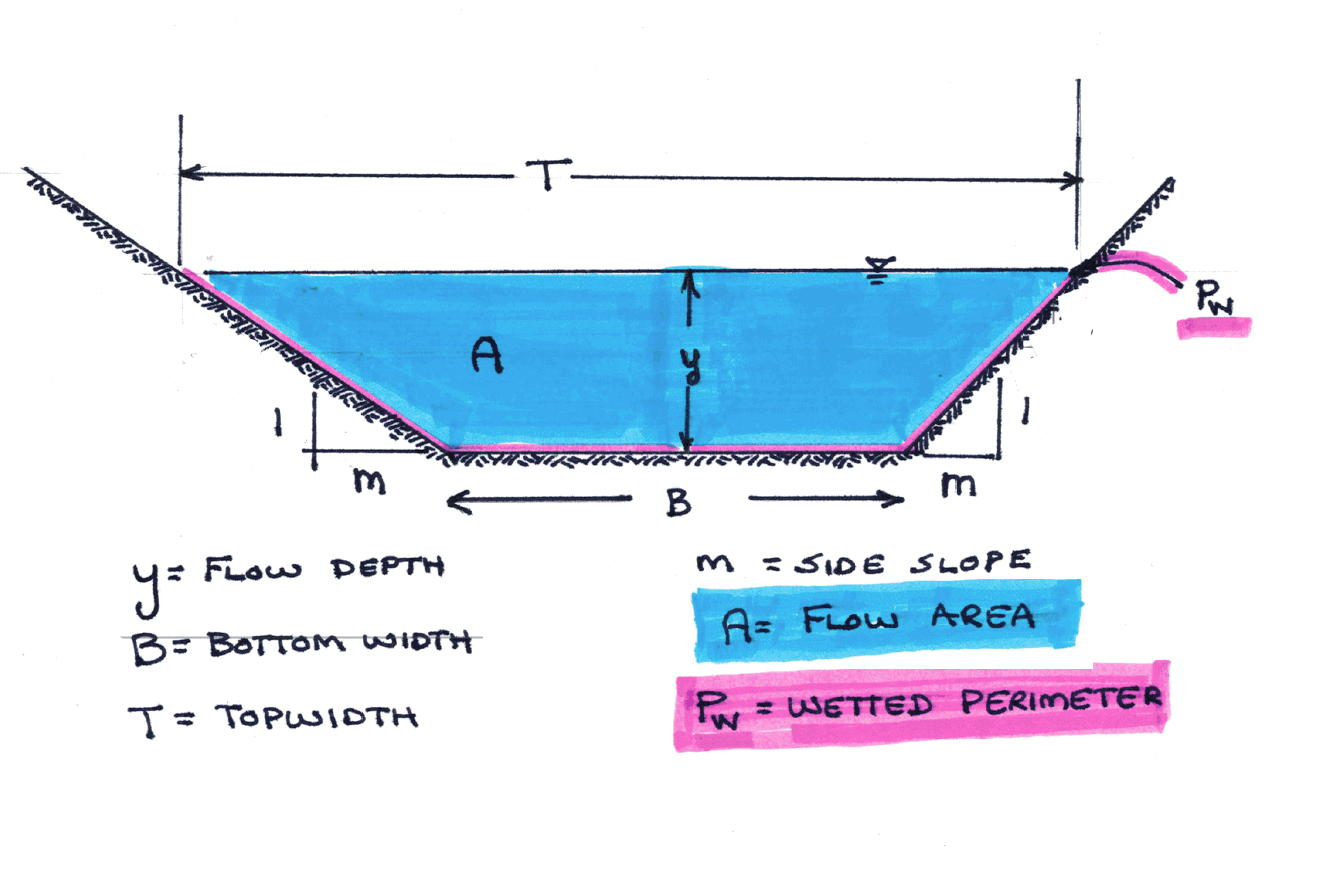
\includegraphics[height=3in]{TrapezoidChannelUS.jpg} 
   \caption{Definition Sketch for a Trapezoidal Channel}
   \label{fig:TrapezoidChannelUS.jpg}
\end{figure}

\begin{equation}
A_{\text{trap.}}(y) = B y + \frac{y^2}{m}
\end{equation}
\begin{equation}
T_{\text{trap.}}(y) = B + 2 \frac{y}{m}
\end{equation}
\begin{equation}
P_{w~\text{trap.}}(y) = B+2y\sqrt{1+\frac{1}{m^2}}
\end{equation}
\clearpage

\begin{tabular}{p{6in}}
~\\ \hline
\end{tabular}

Depth-Area, -Topwidth, -Perimeter for Circular Conduit
\begin{figure}[h!] %  figure placement: here, top, bottom, or page
   \centering
   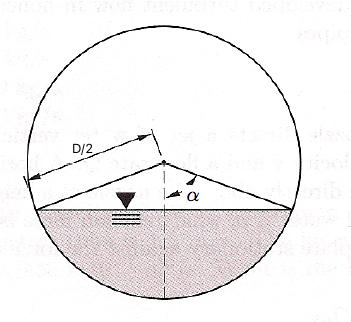
\includegraphics[width=2in]{CircularSewer.jpg} 
   \caption{Definition Sketch for a Circular Conduit}
   \label{fig:CircularSewer.jpg}
\end{figure}
\begin{equation}
\alpha_{\text{circ.}}(y) = cos^{-1}(1-\frac{2y}{D})
\end{equation}
\begin{equation}
A_{\text{circ.}}(y) = \frac{D^2}{4}(\alpha - sin\alpha~cos\alpha)
\end{equation}
\begin{equation}
T_{\text{circ.}}(y) = D~sin\alpha
\end{equation}
\begin{equation}
P_{w~\text{circ.}}(y) = D~\alpha
\end{equation}

\begin{tabular}{p{6in}}
~\\ \hline
\end{tabular}

%%%%%%%%%%%%%%%%%%%%%%%%%%%
\begin{figure}[h!] %  figure placement: here, top, bottom, or page
   \centering
   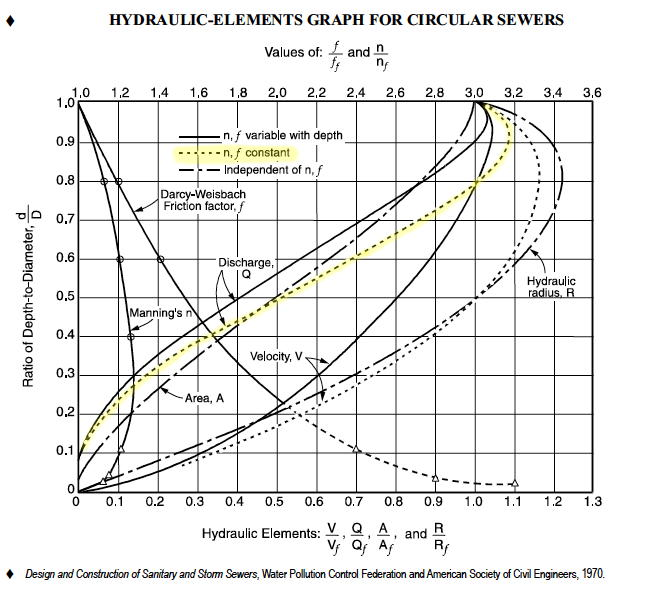
\includegraphics[width=6in]{hydraulic-element-chart.jpg} 
   \caption{Hydraulic element chart for a circular conduit}
   \label{fig:hydraulic-element-chart.jpg}
\end{figure}


\end{document}  




